\documentclass[border=6pt]{standalone}
\usepackage{fontspec,unicode-math}
\setmainfont{Noto Serif}
\setmathfont{STIXTwoMath-Regular.otf}
\usepackage{tikz}
\usetikzlibrary{arrows.meta,calc,patterns,decorations.markings,decorations.pathmorphing,decorations.pathreplacing}
\tikzset{lev/.style={line width=1.18pt,line cap=butt},
 fine/.style={line width=.55pt},light/.style={line width=.4pt},
 curve/.style={line width=1.18pt,line cap=round,line join=round},
 ax/.style={line width=.62pt,-{Latex[length=2.15mm,width=1.2mm]}},
 ray/.style={line width=.64pt,-{Latex[length=1.9mm,width=1.0mm]}},
 dim/.style={line width=.52pt,{Latex[length=1.65mm,width=.85mm]}-{Latex[length=1.65mm,width=.85mm]}},
 flow/.style={line width=.60pt,postaction={decorate},decoration={markings,mark=at position .62 with {\arrow{Latex[length=1.9mm,width=1.0mm]}}}},
 lab/.style={font=\fontsize{13}{16}\selectfont,inner sep=1.5pt},
 small/.style={font=\fontsize{11.2}{13.5}\selectfont,inner sep=1.2pt},
 panel/.style={font=\fontsize{13}{16}\selectfont\itshape,inner sep=1.5pt}}
\pagestyle{empty}
\begin{document}
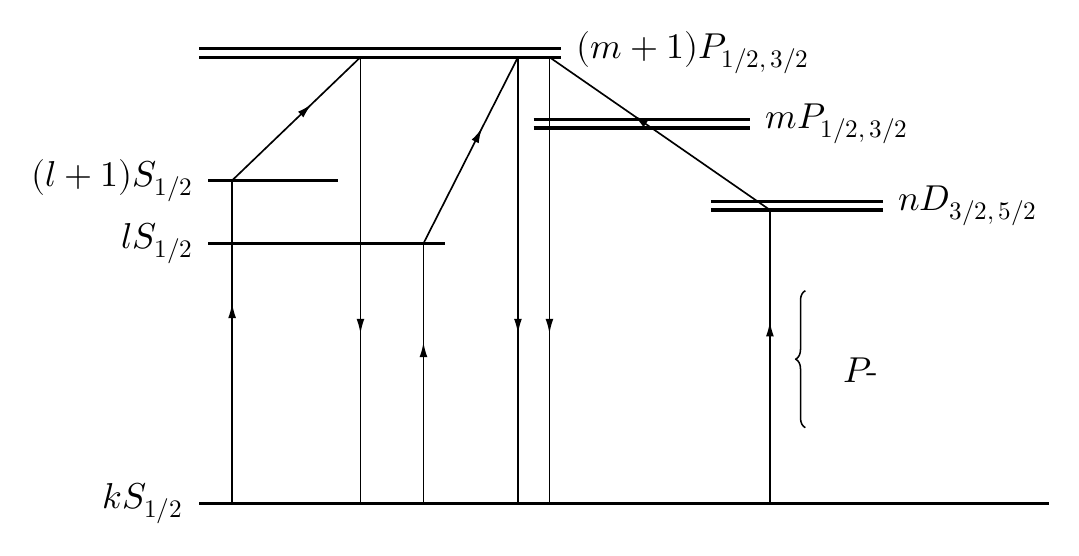
\begin{tikzpicture}[x=1cm,y=1cm,line join=round]
% CP15: One arrowhead per distinct transition; 3 duplicate arrow marks removed.
% Each P0/P1/P2 path retains two upward edges and one downward return.
% Shared state heights are schematic; no atomic energy values inferred.
\draw[lev] (0.000000,0.000000)--(10.800000,0.000000);
\node[lab,anchor=east] at (-0.130000,0.000000) {$kS_{1/2}$};
\draw[lev] (0.120000,3.300000)--(3.120000,3.300000);
\node[lab,anchor=east] at (0.000000,3.300000) {$lS_{1/2}$};
\draw[lev] (0.120000,4.100000)--(1.770000,4.100000);
\node[lab,anchor=east] at (0.000000,4.100000) {$(l+1)S_{1/2}$};
\draw[lev] (0.000000,5.665000)--(4.600000,5.665000);
\draw[lev] (0.000000,5.775000)--(4.600000,5.775000);
\node[lab,anchor=west] at (4.740000,5.720000) {$(m+1)P_{1/2,\,3/2}$};
\draw[lev] (4.250000,4.765000)--(7.000000,4.765000);
\draw[lev] (4.250000,4.875000)--(7.000000,4.875000);
\node[lab,anchor=west] at (7.140000,4.820000) {$mP_{1/2,\,3/2}$};
\draw[lev] (6.500000,3.725000)--(8.680000,3.725000);
\draw[lev] (6.500000,3.835000)--(8.680000,3.835000);
\node[lab,anchor=west] at (8.820000,3.780000) {$nD_{3/2,\,5/2}$};
\coordinate (P0-0) at (0.420000,0.000000);
\coordinate (P0-1) at (0.420000,4.100000);
\coordinate (P0-2) at (2.050000,5.665000);
\draw[flow] (P0-0)--(P0-1);
\draw[flow] (P0-1)--(P0-2);
\draw[flow] (2.050000,5.665000)--(2.050000,0.000000);

\coordinate (P1-0) at (2.850000,0.000000);
\coordinate (P1-1) at (2.850000,3.300000);
\coordinate (P1-2) at (4.050000,5.665000);
\draw[flow] (P1-0)--(P1-1);
\draw[flow] (P1-1)--(P1-2);
\draw[flow] (4.050000,5.665000)--(4.050000,0.000000);

\coordinate (P2-0) at (7.250000,0.000000);
\coordinate (P2-1) at (7.250000,3.725000);
\coordinate (P2-2) at (4.450000,5.665000);
\draw[flow] (P2-0)--(P2-1);
\draw[flow] (P2-1)--(P2-2);
\draw[flow] (4.450000,5.665000)--(4.450000,0.000000);

\draw[fine,decorate,decoration={brace,amplitude=3.5pt}] (7.7,0.96)--(7.7,2.7);
\node[lab,align=left,anchor=west] at (8.120000,1.820000) {Группы\\$P$-состояний};

\end{tikzpicture}
\end{document}
